\documentclass[a4paper]{article}

\usepackage[portuguese]{babel}
\usepackage[utf8]{inputenc}
\usepackage{indentfirst}
\usepackage{graphicx}
\usepackage{verbatim}
\usepackage{caption}
\usepackage{subcaption}
\usepackage{wrapfig}
\usepackage{ragged2e}
\usepackage{listings}
\usepackage{float}

\begin{document}

\setlength{\textwidth}{16cm}
\setlength{\textheight}{22cm}

\title{\Huge\textbf{Eximo}\linebreak\linebreak\linebreak
\Large\textbf{Relatório Intercalar}\linebreak\linebreak
\linebreak\linebreak

\includegraphics[scale=0.1]{res/feup-logo.png}\linebreak\linebreak
\linebreak\linebreak
\Large{Mestrado Integrado em Engenharia Informática e Computação} \linebreak\linebreak
\Large{Programação em Lógica}\linebreak
}

\author{\textbf{Grupo 04: Eximo}\\
Henrique Manuel Martins Ferrolho -  201202772\\
João Filipe Figueiredo Pereira - 201104203 \\
\linebreak\linebreak \\
 \\ Faculdade de Engenharia da Universidade do Porto \\ Rua Roberto Frias, s\/n, 4200-465 Porto, Portugal \linebreak\linebreak\linebreak
\linebreak\linebreak\vspace{1cm}}

\maketitle
\thispagestyle{empty}

%************************************************************************************************
%************************************************************************************************

\newpage

%Todas as figuras devem ser referidas no texto. %\ref{fig:codigoFigura}
%
%%Exemplo de código para inserção de figuras
%%\begin{figure}[h!]
%%\begin{center}
%%\includegraphics[height=1.5cm,width=1.5cm]{white_piece.png}
%%\caption{Peça Branca - Jogador 1}
%%\label{fig:1}
%%\end{center}
%%\end{figure}
%%\includegraphics[scale=0.5]{path relativo da imagem}
%%\includegraphics[scale=•]{•} relativo da imagem}

%%\begin{figure}[h!]
%%\centering
%%\includegraphics[height=1.5cm,width=1.5cm]{white_piece.png}
%%\caption{Peça Branca}
%%\label{fig:whitePiece}
%%\end{figure}

%%\hfill

%%\begin{figure}[h!]
%%\centering
%%
\includegraphics[height=1.5cm,width=1.5cm]{black_piece.png}
%%\caption{Peça Preta}
%%\label{fig:blackPiece}
%%\end{figure}

%%\hfill

%%\begin{figure}[h!]
%%\centering
%%\includegraphics[height=3cm,width=3cm]{board.png}
%%\caption{Tabuleiro}
%%\label{fig:board}
%%\end{figure}




%
%
%\textit{Para escrever em itálico}
%\textbf{Para escrever em negrito}
%Para escrever em letra normal
%``Para escrever texto entre aspas''
%
%Para fazer parágrafo, deixar uma linha em branco.
%
%Como fazer bullet points:
%\begin{itemize}
	%\item Item1
	%\item Item2
%\end{itemize}
%
%Como enumerar itens:
%\begin{enumerate}
	%\item Item 1
	%\item Item 2
%\end{enumerate}
%
%\begin{quote}``Isto é uma citação''\end{quote}

\newpage

%%%%%%%%%%%%%%%%%%%%%%%%%%
\section{O Jogo Eximo}
%%Descrever detalhadamente o jogo, a sua história e, principalmente, as suas regras.
%%Devem ser incluidas imagens apropriadas para explicar o funcionamento do jogo.
%%Devem ser incluidas as fontes de informação (e.g. URLs em rodapé).

\large{\textbf{História}}
\begin{small}

Eximo é um jogo de tabuleiro da família das Damas, concebido em 1 de Fevereiro de 2013.\newline
\end{small}

\large{\textbf{Detalhes do Jogo}}
\begin{small}

O jogo realiza-se num tabuleiro de dimensões 8x8, em que as casas têm todas cores semelhantes. Cada jogador começa com 16 peças colocadas em locais pré-definidos no respectivo lado do tabuleiro, como mostra a imagem abaixo.\newline

\begin{figure}[h!]
  \begin{minipage}[h!]{0.2\textwidth}
    \includegraphics[width=0.4\textwidth]{res/white_piece.png}
    \centering
    \caption{Peça branca}
    \label{fig:2}
  \end{minipage}
	\quad\quad\quad
  \begin{minipage}[h!]{0.2\textwidth}
    \includegraphics[width=\textwidth]{res/board.png}
    \caption{Tabuleiro}
    \label{fig:3}
  \end{minipage}
	\quad\quad\quad
  \begin{minipage}[h!]{0.2\textwidth}
    
\includegraphics[width=0.4\textwidth]{res/black_piece.png}
	\centering
    \caption{Peça preta}
    \label{fig:4}
  \end{minipage}
\end{figure}

No jogo, as movimentações e as capturas podem ser ortogonais ou diagonais. Há apenas um tipo de peça: os homens. Os homens podem saltar sem efectuar captura. Quando um homem atinge a última linha, ocorre a libertação de outro homem.
\end{small}\newline

\large{\textbf{Objectivo}}
\begin{small}

O objectivo do jogo é, tal como nas Damas, \textbf{capturar todas as peças} do oponente, saltando sobre elas, ou \textbf{incapacitar o adversário} de realizar qualquer movimento.
\end{small}\newline

\large{\textbf{Jogada}}
\begin{small}

Em cada jogada, um jogador pode fazer uma de duas acções: \textbf{mover ou capturar}.
\end{small}\newline

\large{\textbf{Movimento}}
\begin{small}

Uma peça pode mover-se em três direcções: para a frente ou na diagonal (\textbf{norte, nordeste ou noroeste}). Numa jogada, o movimento nunca pode ser efectuado para a retaguarda. 

Existem dois tipos de movimentos: \textbf{Normal e Salto}. 
\begin{itemize}
\item \textbf{Movimento Normal}:
uma peça move-se para uma \textbf{casa adjacente e vazia}. 
\item \textbf{Movimento em Salto}:
\textbf{uma peça salta sobre uma peça aliada adjacente, se e só se a casa correspondente} (ao lado da peça aliada) \textbf{estiver vazia}, colocando assim a peça nessa casa. Se a mesma peça do jogador puder continuar a realizar o mesmo movimento de salto sobre outra peça amigável então terá de o fazer. \textbf{Durante um movimento de salto a peça não pode capturar peças inimigas}.

Quando existe \textbf{mais do que uma forma de saltar}, o jogador \textbf{pode escolher a peça que irá usar para executar o salto}, bem como o tipo de salto ou sequência de saltos a fazer. Não é obrigatório que a sequência de saltos escolhida pelo jogador seja aquela que possui o maior número de saltos; porém, \textbf{após escolher uma sequência, o jogador deve executar todos os saltos possíveis}.
\end{itemize}
\end{small}

\begin{figure}[h!]
  \begin{minipage}[h!]{0.3\textwidth}
    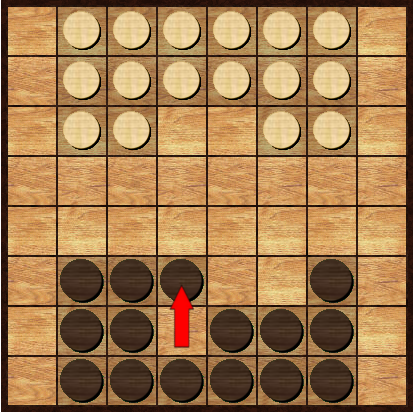
\includegraphics[width=\textwidth]{res/normalMove.png}
    \caption{Movimento Normal}
    \label{fig:5}
  \end{minipage}
\quad\quad\quad\quad\quad\quad\quad\quad
  \begin{minipage}[h!]{0.3\textwidth}
    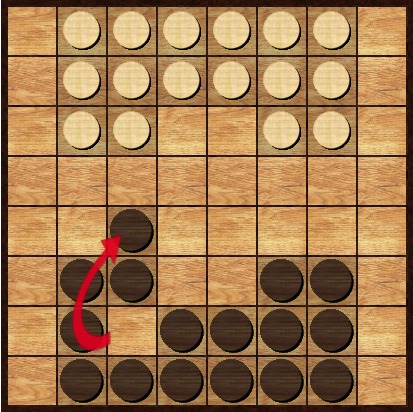
\includegraphics[width=\textwidth]{res/jumpMove.png}
    \caption{Movimento em Salto}
    \label{fig:6}
  \end{minipage}
  \caption{Movimentos}
\end{figure}

\large{\textbf{Captura}}
\begin{small}

Um \textbf{jogador pode capturar} em cinco direcções: \textbf{frente}, \textbf{diagonal para a frente}, \textbf{direita} ou \textbf{esquerda} (norte, nordeste, noroeste, este ou oeste). 

\begin{itemize}
\item \textbf{Captura}:
um jogador \textbf{salta sobre uma peça adjacente do adversário}, se a \textbf{próxima casa}, na mesma direcção, \textbf{estiver vazia}, colocando, assim, a peça sobre essa casa. A \textbf{peça do oponente é removida do tabuleiro}. Se a \textbf{peça} do mesmo jogador \textbf{puder continuar a capturar outras peças do adversário}, então \textbf{deve fazê-lo}. A \textbf{captura é obrigatória} e deve continuar enquanto for possível.
\end{itemize}

\begin{figure}[h!]
  \begin{minipage}[h!]{0.3\textwidth}
    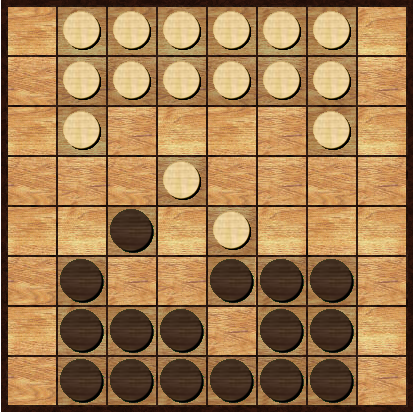
\includegraphics[height=5cm,width=5cm]{res/captureMove.png}
    \caption{Estado anterior à captura}
    \label{fig:7}
  \end{minipage}
	\quad\quad\quad\quad\quad\quad\quad
  \begin{minipage}[h!]{0.3\textwidth}
    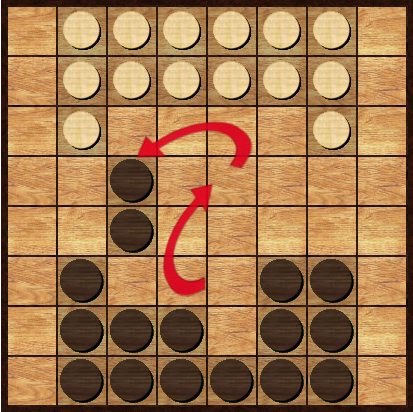
\includegraphics[height=5cm,width=5cm]{res/captureMoveResult.png}
    \caption{Estado posterior à captura}
    \label{fig:8}
  \end{minipage}
\end{figure}

Tal como no \textbf{Movimento de Salto}, \textbf{o jogador escolhe} livremente \textbf{qual a sequência de saltos a efectuar}.
\end{small}\newline

\large{\textbf{Última Linha}}
\begin{small}

Quando uma peça atinge a extremidade do tabuleiro, essa peça é removida de imediato e o jogador recebe dois movimentos extra para efectuar nesse mesmo momento: colocar duas peças novas numa casa vazia localizada nas duas primeiras linhas, à excepção das quatro casas laterais (duas do lado esquerdo, e duas do lado direito).
\end{small}\newline

%%%%%%%%%%%%%%%%%%%%%%%%%%
\section{Representação do Estado do Jogo}

%Descrever a forma de representação do estado do tabuleiro (tipicamente uma lista de %listas), com exemplificação em Prolog de posições iniciais do jogo, posições %intermédias e finais, acompanhadas de imagens ilustrativas.

Representação do estado inicial do tabuleiro:
\begin{small}
\begin{lstlisting}
[[empty, white, white, white, white, white, white, empty],
 [empty, white, white, white, white, white, white, empty],
 [empty, white, white, empty, empty, white, white, empty],
 [empty, empty, empty, empty, empty, empty, empty, empty],
 [empty, empty, empty, empty, empty, empty, empty, empty],
 [empty, black, black, empty, empty, black, black, empty],
 [empty, black, black, black, black, black, black, empty],
 [empty, black, black, black, black, black, black, empty]]
\end{lstlisting}
\end{small}
\begin{figure}[h!]
	\centering
    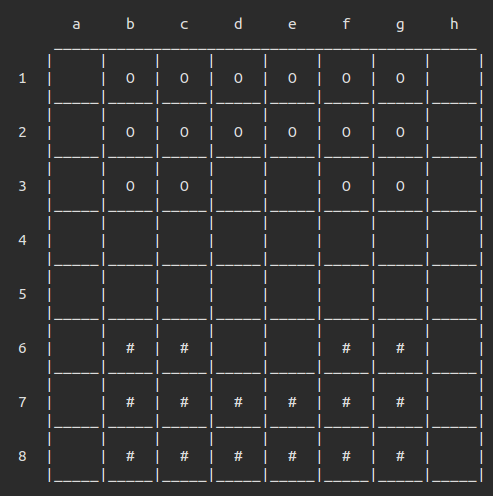
\includegraphics[height=5cm,width=5cm]{res/initialBoard.png}
    \caption{Estado inicial do tabuleiro visualizado na consola}
    \label{fig:9}
\end{figure}

\pagebreak
Representação de um possível estado intermédio do tabuleiro:
\begin{small}
\begin{lstlisting}
[[empty, white, white, white, white, white, white, empty],
 [empty, white, white, empty, white, white, white, empty],
 [empty, white, white, white, empty, white, white, empty],
 [empty, empty, empty, empty, empty, empty, empty, empty],
 [empty, empty, black, empty, empty, empty, empty, empty],
 [empty, black, black, black, empty, black, black, empty],
 [empty, black, empty, empty, black, black, black, empty],
 [empty, black, black, black, black, black, black, empty]]
\end{lstlisting}
\end{small}
\begin{figure}[h!]
	\centering
    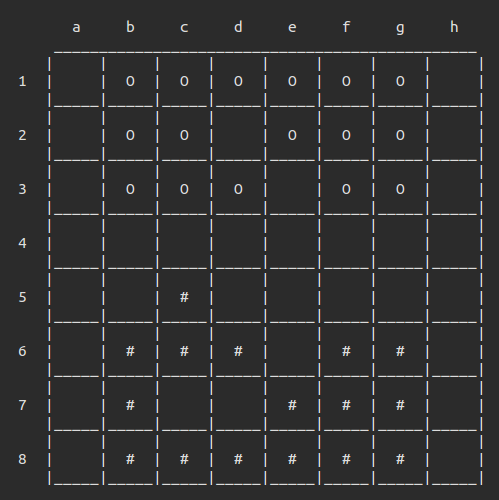
\includegraphics[height=5cm,width=5cm]{res/intermedialBoard.png}
    \caption{Estado intermédio do tabuleiro visualizado na consola}
    \label{fig:9}
\end{figure}

Representação de um possível estado final do tabuleiro:
\begin{small}
\begin{lstlisting}
[[empty, empty, empty, empty, empty, empty, empty, empty],
 [empty, empty, empty, empty, empty, empty, empty, empty],
 [empty, empty, empty, empty, empty, empty, empty, empty],
 [empty, empty, empty, empty, empty, empty, empty, empty],
 [empty, empty, empty, empty, empty, empty, empty, empty],
 [empty, empty, empty, empty, empty, empty, empty, empty],
 [empty, empty, empty, white, empty, empty, empty, empty],
 [empty, empty, black, black, black, empty, empty, empty]]
\end{lstlisting}
\end{small}
\begin{figure}[h!]
	\centering
    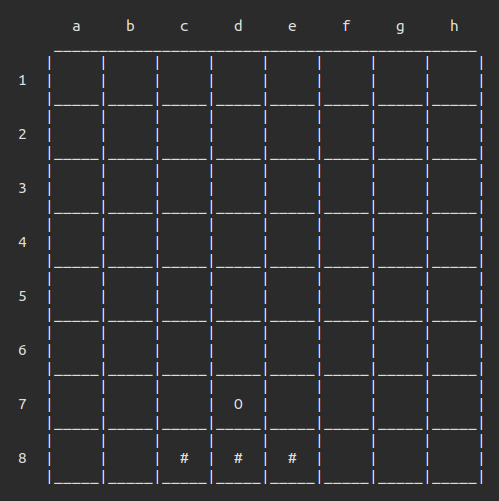
\includegraphics[height=5cm,width=5cm]{res/finalBoard.png}
    \caption{Estado final do tabuleiro visualizado na consola}
    \label{fig:9}
\end{figure}

\pagebreak
%%%%%%%%%%%%%%%%%%%%%%%%%%
\section{Visualização do Tabuleiro}

%Descrever a forma de visualização do tabuleiro em modo de texto e o(s) predicado(s) %Prolog construídos para o efeito.
%Deve ser incluída pelo menos uma imagem correspondente ao output produzido pelo %predicado de visualização.

\begin{small}
De seguida está apresentado o código que, em princípio, será usado para mostrar o tabuleiro na consola.
\end{small}

\begin{small}
\begin{lstlisting}
%=================%
%= Board drawing =%
%=================%
printColumnIdentifiers:-
	write('        a     b     c     d     e     f     g     h').

rowIdentifiersList(['  1  ', '  2  ', '  3  ', '  4  ', '  5  ', '  6  ', '  7  ', '  8  ']).

printInitialSeparator:-
	write('      _______________________________________________').

createSeparatorN(0, _, []).
createSeparatorN(N, SS, [SS | Ls]):-
	N1 is N-1,
	createSeparatorN(N1, SS, Ls).

printBoardRowValues([]).
printBoardRowValues([Head | Tail]):-
	cell(Head, Piece),
	write('  '), write(Piece), write('  |'),
	printBoardRowValues(Tail).

printBoardRow([], []).
printBoardRow(Line, RowIdentifiersListHead):-
	length(Line, Length),
	createSeparatorN(Length, '_____|', Separator),
	createSeparatorN(Length, '     |', Separator2),
	write('     '), write('|'), printList(Separator2), nl,
	write(RowIdentifiersListHead), write('|'), printBoardRowValues(Line), nl,
	write('     '), write('|'), printList(Separator), nl.

printRemainingBoard([], []).
printRemainingBoard([Line | Tail],
	[RowIdentifiersListHead | RowIdentifiersListTail]):-
	printBoardRow(Line, RowIdentifiersListHead),
	printRemainingBoard(Tail, RowIdentifiersListTail).

printBoard([Line | Tail]):-
	printColumnIdentifiers, nl,
	printInitialSeparator, nl,
	rowIdentifiersList(RowIdentifiers),
	printRemainingBoard([Line | Tail], RowIdentifiers), nl.
\end{lstlisting}
\end{small}

\begin{small}
A figura 9, 10 e 11 - apresentadas anteriormente - representam os outputs esperados para a consola do estado inicial, intermédio e final do tabuleiro, respectivamente, produzidos pelo código acima apresentado.
\end{small}

\pagebreak
%%%%%%%%%%%%%%%%%%%%%%%%%%
\section{Movimentos}

Cabeçalho do predicado de movimentação de uma peça:\newline
\begin{small}
movePiece(Row, Column, DestRow, DestColumn, Board)
\end{small}\newline

Cabeçalho do predicado de captura de uma peça:\newline
\begin{small}
capturePiece(Row, Column, Board)
\end{small}

\end{document}
